\section{Sensor}
Sensoren der anvedes er en "Line Sensor Breakout - QRE1113" fra sparkfun.com. Det er en analog sensor som sidder på et breakout board i en spændingsdeling. Dette betyder at der blot skal aflæses spænding på en pin for at få en værdi der svare til en lysstyrke fra sensoren.

\begin{figure}[h!]
  \centering
  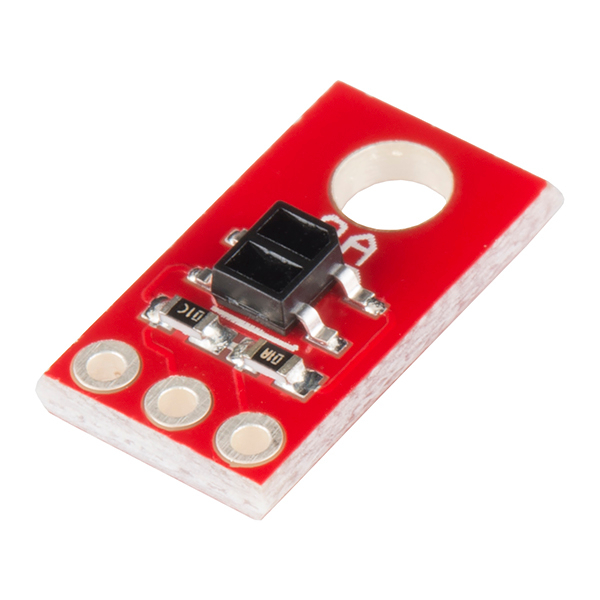
\includegraphics[width=0.3\textwidth]{figures/lyssensor.png}
\end{figure}

Dimensionerne for sensoren er 0.30 x 0.55 “ (7.62 x 13.97 mm) \fxnote{Måske skal det værr i billede teksten.}
\newline
Specifikationerne er \fxnote{Måske skal det stå i punkt form.} 
\newline
5VDC operating voltage
25mA supply current
Optimal sensing distance: 0.125" (3mm)

Kilde (Sparkfun.com)
\newline
For at kunne anvende lyssensoren med en arduino skal der ikke anvendes meget kode. Sensoren sidder i en spændingsdeling og outputtet fra lyssensoren bliver tilkoblet en pin på arudinoen. Så skal der blot foretages en analog måling med ADC'en på arduoen. 
Dette gøres ved at bruge analogRead() i softwaren.
\newline

Inde i lys-sensoren sidder der en transistor i en spændingsdeling. Denne transistor kan generere noget høj frekvent støj. Dette filtrers væk med et low-pass filter.